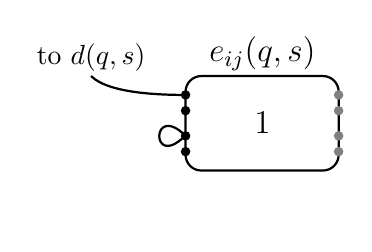
\begin{tikzpicture}[baseline=(X.base),scale=0.8]
\node at (0,0) (X){};

\begin{scope}[xshift=0cm]       
\draw[rounded corners=2mm,thick] (0,0) rectangle (2.43cm,1.5 cm);  
  \foreach \x /\color in {0/black,2.43/gray}
{     \foreach \y in {1.2,.95,.55,.3}
{       \draw[fill=\color,draw=\color] (\x cm, \y cm) circle (.66mm);
    }} 
\node at (1.22cm, .75cm) {\large{$1$}};   
 \node at (1.22cm, 1.85cm){\large{$e_{ij}(q,s)$}};
\draw[thick,looseness=.66] (0cm,1.2cm) to [out=180,in=-45] (-1.5cm,1.5cm);
\node at (-1.5,1.8){to $d(q,s)$};
\draw[thick,looseness = 200] (0,0.55) to [out = 135, in = 225] (-.01,0.55);
\end{scope}
\node at (0,-0.7){};
\end{tikzpicture}